\documentclass{aims}

%%%%%%%%%%%%%%%%%%%%%%%%%%%%%%%%%%%%%%%%%%
\usepackage{txfonts}
\def\typeofarticle{Type of article}
\def\currentvolume{5}
\def\currentissue{x}
\def\currentyear{2019}
\def\currentmonth{Received date 1 July 2016, Accepted date 6 September}
\def\ppages{xxx--xxx}
\def\DOI{}
\def\Received{xx 2019}
\def\Accepted{xx 2019}
\def\Published{xx 2019}


\newcommand{\ep}{\varepsilon}
\newcommand{\eps}[1]{{#1}_{\varepsilon}}

\numberwithin{equation}{section}
\DeclareMathOperator*{\essinf}{ess\,inf}


\begin{document}
\global\long\def\pardiff#1#2{\frac{\partial#1}{\partial#2}}%

\title{Estimation of Vital Parameters of Glioblastoma Multiforme Growth Dynamics from a Model with Explicit Birth and Death Rates}

\author{%
  Lifeng Han\affil{1},
  Steffen Eikenberry\affil{1},
  Changhan He\affil{1},
  Lauren Johnson\affil{1},
  Mark Preul\affil{2},
  Eric Kostelich \affil{1},
  and
  Yang Kuang\affil{1,} \corrauth
}

% \shortauthors is used in copyright information in the end of the paper
\shortauthors{the Author(s)}

\address{%
  \addr{\affilnum{1}}{School of Mathematical and Statistical Sciences, Arizona State University, Tempe, AZ 85287, USA}
  \addr{\affilnum{2}}{Department of Neurosurgery Research, Barrow Neurological Institute, St. Joseph’s Hospital and Medical Center, Phoenix, AZ 85013, USA}}

% corresponding author
\corraddr{kuang@asu.edu}

\begin{abstract}
Glioblastoma multiforme (GBM) is an aggressive brain cancer with grim
prognosis. Its morphology is characterized by layered structure, i.e.,
an inner necrotic core and an outer rim of proliferating cells. This
structure can be observed in magnetic resonance images. A mathematical
model of GBM growth with explicit birth and death rate is proposed.
This model generates a traveling wave which mimic the cancer progression. 
We develop some novel methods to approximate key characteristics of 
the wave profile, which can be compared with image data. Several simplistic 
forms of growth and death terms and their parameter identifiability are 
studied. We use image data of GBM patients to get personalized parameterization 
of the model, of which the biological and clinical implications are discussed. 
\end{abstract}

\keywords{Glioblastoma multiforme modeling; parameter estimation; traveling wave; necrosis; proliferation}

\maketitle

\section{Introduction}

Glioblastoma multiforme (GBM) is a type of the most aggressive brain
cancer. Patients with GBM have a mean survival length less than 15
months from the time of diagnosis \cite{Norden2006}. Its fast progression
is characterized by highly proliferating and invasive cancer cells.
The information on individual GBM patients are very scarce while challenges 
to treat GBM are numerous. A key piece of information clinical doctors may 
have for their GBM patients are MRI images. Often there is only one image 
that lead to the diagnosis and the patients are immediately scheduled for 
surgery. The main questions for surgeons are how much and where to cut and 
how soon the cancer will emerge and where. These are decades old questions 
that surface in other type of cancer treatments. 

GBM morphology manifests a layered structure: there is a necrotic
core at the center, a band of proliferating cells at the outer rim
and a transition layer of quiescent cancer cells in between. GBM
can be visualized by magnetic resonance (MR) imaging, which is commonly
used to inform clinical decisions. One of the hallmarks of cancer in 
general, and GBM in particular, is its heterogeneity between individual 
patients. This heterogeneity imposes a challenge to GBM treatment. 

Appropriate mathematical models may offer a way to tackle this challenge. 
Mathematical modeling has already provided many valuable insights to our 
understanding of cancer and its treatment \cite{Kuang}. Mathematical models 
on GBM are formulated to provide new tools for studying the growth of gliomas and for practical applications (see \cite{GBMreview} for a review). A popular type of those models oftem takes the form of a system of reaction-diffusion equations. In many cases \cite{Harley2014,Gerlee2016,Stepien2018},
those systems generate a traveling wave solution of which the speed
is of great interests since it is related to how fast cancer progresses. 

However, models which confront the heterogeneity of GBM directly by
utilizing spatiotemporal patient-specific data are rare. Swanson
and her collaborators \cite{Swanson2008,Neal2013,Jackson2015a} is
one of the few teams which focus on this endeavor. They employed 
variants of the well-known Fisher's equation to study cancer cells'
proliferation (P) and invasion (I) dynamics \cite{FISHER1937} 
(hence called PI model in \cite{Jackson2015a})
and parameterized it using patient MR images. The estimated proliferation
and diffusion parameters and a model-derived metric called days gained
are deemed to be instrumental to clinical treatments. 

Treating the cancer cells as a single species can be a gross simplification and
by doing so the structured morphology of GBM is lost. Although there are modeling 
efforts taking into account of multi-species nature of cancer cells \cite{Eikenberry2009,Swanson2011}, they are usually too complicated to be 
practically useful given scarcity of patient specific images. 

For most GBM patients and their doctors, available MRI images maybe all taken
at the same day or at just two different days. Practical modeling efforts must be constrained by such brutal data limitation and formulate models which can be parameterized with the images at hand. Recognizing this reality, we propose a model 
which includes two species of cancer cells, i.e., proliferating and quiescent,
and is capable of exploiting the structural information offered by only
one or two MRI images. 

Gliomas can only be imaged indirectly on MRI, and are typically characterized,
on T1-weighted sequences, by a large, often necrotic core region surrounded
by a bright enhancing rim that correlates with high blood vessel density
and (presumably) rapid cell proliferation. This core and
rim is usually surrounded by a large expanse of edema that is visible
on T2-weighted MRI, and may represent diffusely invasive, highly motile
GBM cells. Thus, we have three digital marks from imaging: necrotic radius,
enhancing radius, and T2 (or maximum) radius. We hypothesize that a relatively 
simple mathematical model framework may capture all these three
digital marks, and yield insights into the relative contributions of cellular
proliferation, motility, and necrosis to the observed image features.

The paper is organized as following. We first describe our model and
its assumptions. Then we demonstrate that the model has a traveling
wave solution and present the approximate wave profile. We devise
a simple procedure to estimate patient-specific parameters by fitting the approximate
wave profile to that of patient images. Identifiability of parameters is also 
discussed. Moreover, we apply this parameter estimation procedure to 
obtain the cancer vital dynamics parameters (consisting of the rate of cancer cell proliferation, death and diffusion) for several patients.  



\section{Model and method}
\subsection{Model description}
To model the growth of GBM, we propose a system of reaction-diffusion
equations 

\begin{subequations}\label{eq:main3d}
\begin{eqnarray}
\pardiff pt & = & \nabla\cdot\bigg[\frac{Dp}{p+q}\nabla(p+q)\bigg]+\tilde{g}(w)p-\tilde{\delta}(w)p,\\
\pardiff qt & = & \nabla\cdot\bigg[\frac{Dq}{p+q}\nabla(p+q)\bigg]+\tilde{\delta}(w)p,
\end{eqnarray}
\end{subequations}where two species are considered: proliferating
cells and quiescent cells whose density at time $t$ and location
$x$ is represented by $p(x,t)$ and $q(x,t)$ respectively. We assume
the flux of total population due to migration is $-D\nabla(p+q)$
where $D$ is a constant diffusion coefficient. It is further assumed
that the proportion of the total flux contributed by each species
equals their proportion of the total population. This diffusion term
is believed to be a realistic account of cancer cell movements \cite{Sherratt2001}. 

Per capita birth rate is $\tilde{g}(w)$ and the proliferating cells
become quiescent with per capita rate $\tilde{\delta}(w)$. Both of
them are functions of $w$. We define $w=1-p-q$, interpreted as availability
of space or some generic nutrient (we call it growth factor henceforth).
By doing so, we have scaled the maximum cell density to be 1. In our
model, necrosis is not explicitly included but can be regarded as being
lumped into $q$. This choice is supported by the fact that MR only
visualizes proliferating cells and does not distinguish between quiescence
and necrosis. Our motivation of keeping the model simple enough is to estimate 
model parameters based on information that can be provided by the images. 
Note that quiescent cells can not become proliferating
again but only turns into necrosis. Therefore $\tilde{\delta}(w)$
can be viewed as death rate. 

In order to make the model biologically reasonable, we impose the following constraints
on $g(w)$ and $\delta(w)$: 
\begin{equation}
\tilde{g}'(w)\ge0,\tilde{\delta}'(w)\le0,\tilde{g}(1)\ge\tilde{\delta}(1)=0,\tilde{\delta}(0)>\tilde{g}(0)=0.\label{eq:1st assumption}
\end{equation}
That is, birth/death should increase/decrease with availability of
the growth factor, and there is more birth than death at maximum growth
factor while there is only death and no growth in absence of growth
factor. It is also assumed that death rate is negligible at maximum
growth factor. With these assumptions, it can be shown that the solution
of (\ref{eq:main3d}) stay nonnegtive and is bounded by $p+q\le1$
for all $t$ with the usual suitable initial condition. 

We can only estimate up to three parameters based on the three pieces of information
we can derive from MR images. Therefore we want a few more restrictions
on $\tilde{g}(w)$ and $\tilde{\delta}(w)$ for the ease of parameter
estimation and ensure their identifiability. Since we can only introduce
two more parameters in addition to diffusion coefficient $D$, we
introduce $\rho$ and $k$ into $\tilde{g}(w)$ and $\tilde{\delta}(w)$
respectively and indicate their dependence on the parameters as $\tilde{g}(w;\rho)$
and $\tilde{\delta}(w;k)$. It is desirable to make the proliferating
rate at maximum growth factor be $\rho$
and death rate at zero growth factor
be $k$, i.e., $\tilde{g}(1,\rho)=\rho,\ \tilde{\delta}(0;k)=k$.
For reasons that will become clear later, we pick the functional form
which can be written as $\tilde{g}(w;\rho)=\rho g(w)$ and $\tilde{\delta}(w;k)=k\delta(w)$.
Although we have stated several additional assumptions, it should
be noted that they impose little impact on the generality and flexibility
of our model. The benefit of including them will become clear in the
section of parameter estimation. 

\subsection{Approximate wave profile}
In most biological applications of reaction-diffusion models, solutions quickly take the forms of traveling waves. MRI images of GBM cancer growth suggests we can approximate
the cancer population growth curve by a traveling wave solution of its growth model.
In order to uniquely identify and accurately approximate GBM growth model parameters,
it is highly desirable to obtain some analytic approximation of the travel wave so a 
computational match of the image wave profile and the approximate model wave profile can be made.
To this end and for simplicity, we consider one spatial dimension. It is justified
by the fact that the tumor is mostly spherical and at the time of
diagnosis its radius is large enough so that radial effect is negligible.
Together with the aforementioned assumptions, the equations may take the following forms:

\begin{subequations}\label{eq:main}
\begin{eqnarray}
\pardiff pt & = & \pardiff{}x\bigg[\frac{Dp}{p+q}\pardiff{}x(p+q)\bigg]+\rho g(w)p-k\delta(w)p,\\
\pardiff qt & = & \pardiff{}x\bigg[\frac{Dq}{p+q}\pardiff{}x(p+q)\bigg]+k\delta(w)p.
\end{eqnarray}
\end{subequations}We nondimensionlize the system using the characteristic
length $\sqrt{D/k}$ and the characteristic time $1/k$ so that $x=\sqrt{D/k}\hat{x}$
and $t=\hat{t}/k$, which leads to \begin{subequations}\label{eq:dpdt dqdt}
\begin{eqnarray}
\pardiff p{\hat{t}} & = & \pardiff{}{\hat{x}}\bigg[\frac{p}{p+q}\pardiff{}{\hat{x}}(p+q)\bigg]+\hat{\rho}g(w)p-\delta(w)p,\\
\pardiff q{\hat{t}} & = & \pardiff{}{\hat{x}}\bigg[\frac{q}{p+q}\pardiff{}{\hat{x}}(p+q)\bigg]+\delta(w)p,
\end{eqnarray}
\end{subequations}where $\hat{\rho}=\rho/k$. We are seeking a traveling
wave solution, i.e., $p(\xi)=p(\hat{x}-c\hat{t}),q(\xi)=q(\hat{x}-c\hat{t})$
where $c$ is wave speed.
Substituting these into (\ref{eq:dpdt dqdt}) gives 

\begin{subequations}\label{eq:in wave cord}
\begin{eqnarray}
(\frac{p}{p+q}(p+q)')'+cp'+\hat{\rho}g(w)p-\delta(w)p & = & 0,\\
(\frac{q}{p+q}(p+q)')'+cq'+\delta(w)p & = & 0,
\end{eqnarray}
\end{subequations} where the prime indicates the derivative with
respect to $\xi$. Linearizing at the wave head, i.e., substitute
an ansztz $p=Ae^{-r\xi}$ and $q=Be^{-r\xi}$ into (\ref{eq:in wave cord})
gives $(r^{2}-cr+\rho)A=0$. For biologically realistic wave front, we expect $A>0,\, B>0$ and $r>0$.
This requires that $c^2>4\rho$, which implies that the minimum
speed of the wave $c_{\min}=2\sqrt{\hat{\rho}}$ . It is numerically
verified that the minimum speed is exactly the asymptotic speed, i.e.,
$c=c_{\min}$.

To obtain a approximate wave profile, we adopt a popular method first used
by Canosa in \cite{Canosa1973}. We rescale the wave coordinate $z=-\text{\ensuremath{\xi/c}}$,
which leads to

\begin{subequations}\label{eq:1/c^2}
\begin{eqnarray}
\frac{1}{c^{2}}(\frac{p}{p+q}(p+q)')'-p'+\hat{\rho}g(w)p-\delta(w)p & = & 0,\label{eq:1/c^2a}\\
\frac{1}{c^{2}}(\frac{q}{p+q}(p+q)')'-q'+\delta(w)p & = & 0,\label{eq:1/c^2b}
\end{eqnarray}
\end{subequations}where the prime indicates the derivative with respect
to $z$. Assuming that $1/c^{2}$ is small, we neglect the first terms
of (\ref{eq:1/c^2a}),(\ref{eq:1/c^2b}). Writing the system in terms
of $p$ and $w$, we obtain the following reduced system 

\begin{subequations}\label{eq:pp system}
\begin{align}
\frac{dp}{dz} & =p(\hat{\rho}g(w)-\delta(w)),\label{eq:dpdz}\\
\frac{dw}{dz} & =-\hat{\rho}pg(w),\label{eq:dwdz}
\end{align}
\end{subequations}which is amenable to phase plane analysis. The
approximate wave solution corresponds to a trajectory that leaves
$(0,1)$ and ends at $(0,w^{*})$ with $w^{*}\in[0,1)$ (see Figure
\ref{fig:pp}). Its existence based on assumptions (\ref{eq:1st assumption})
is shown in the appendix. Dividing (\ref{eq:dpdz}) by (\ref{eq:dwdz}) yields 

\begin{equation} \label{eq:dpdw}
\frac{dp}{dw}=\frac{\delta(w)}{\hat{\rho}g(w)}-1.
\end{equation}

 Upon integration we get $p$ as a function of $w$, i.e., $p=p(w)$,
which we will make use of in the next section. 

\begin{figure}
\begin{center}
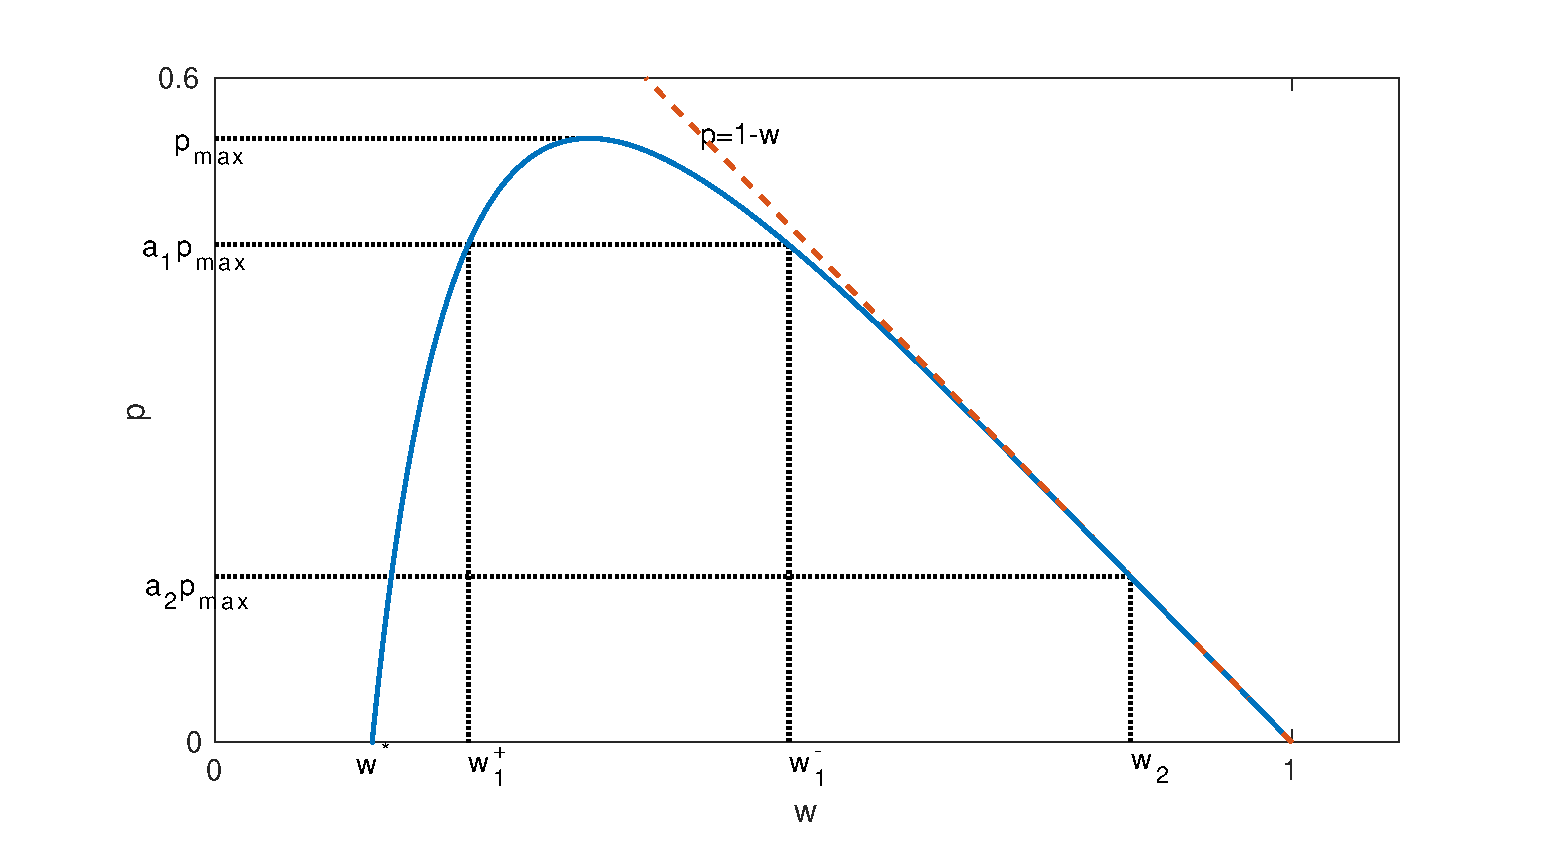
\includegraphics[scale=0.65]{plots/pp.eps}\caption{\label{fig:pp}A typical trajectory that connects (0,1) and $(0,w^*)$ in the phase plane. Given $\delta(w)$ and $g(w)$, this trajectory can be found by integrating (\ref{eq:dpdw}). This trajectory represents an approximate traveling wave solution and its existence under general assumptions is shown in supplemental material.}
\end{center}
\end{figure}

\subsection{Parameter estimation}

We first discuss the three key values which we may obtain
from MR images and use that to fit our model. There are two types of MR: T1
highlights high density of proliferating cells while T2 has a lower
detection threshold. We denote their detection thresholds as $100\times a_{1}\%$
and $100\times a_{2}\%$ of $p_{\max}=\max_{z}\{p(z)\}$ (the actual
maximum density of proliferating cells given by the traveling wave
solution) with $a_{1}>a_{2}$. To fit our 1-D model, we convert necrotic
core volume, T1 volume and T2 volume into equivalent spheres with
their radius denoted by $R_{0},R_{1}$ and $R_{2}$, respectively (to do: figure
needed). Therefore, the width of proliferating rim denoted as $L_{1}$
and $L_{2}$ for T1 and T2 images can be calculated, i.e., $L_{1}=R_{1}-R_{0}$
and $L_{2}=R_{2}-R_{1}$. Typically, there are two MR scans before
surgery: one is at diagnosis and the other is right before surgery
with a usual time interval of a few weeks \cite{Swanson2008}. The
image-derived wave velocity $V$ is the change in tumor radius divided
by the length of this time interval. 

From our approximate wave profile, we can compute the corresponding
quantities to match with images (Figure \ref{fig:Match wid}). The
rim width (in dimensional form) is computed as below

\begin{subequations}
\begin{eqnarray}
\ell_{1} & = & \frac{\sqrt{D\rho}}{k}\int_{w_{1}^{-}}^{w_{1}^{+}}\frac{dz}{dw}dw\label{eq:l1}\\
\ell_{2} & = & \frac{\sqrt{D\rho}}{k}\int_{w_{1}^{+}}^{w_{2}}\frac{dz}{dw}dw,\label{eq:l2}
\end{eqnarray}
\end{subequations}

where $w_{1}^{\pm}$ and $w_{2}$ satisfy $p(w_{1}^{\pm})=a_{1}p_{\text{max}},p(w_{2})=a_{2}p_{\max}$ with $p(w)$ resulted from integration of (\ref{eq:dpdw}). Additionally, model-derived wave
speed $c=2\sqrt{\rho D}$ can be matched with image-derived speed
$V$. Thus we have three nonlinear equations 
\begin{equation}
\{\ell_{1}=L_{1},\ell_{2}=L_{2},c=V\},\label{eq:l1l2c}
\end{equation}
 from which we hope to find parameters $D,\rho$ and $k$. Due
to the assumptions we made before, we can simply take the ratio of
(\ref{eq:l1}) and (\ref{eq:l2}), which gives 
\begin{equation}
f(\hat{\rho})\equiv\frac{\int_{w_{1}^{-}}^{w_{1}^{+}}\frac{dz}{dw}dw}{\int_{w_{1}^{-}}^{w_{1}^{+}}\frac{dz}{dw}dw}=\frac{L_{1}}{L_{2}},\label{eq:f(rho/k)}
\end{equation}
where we note that the integrals are a function of $\hat{\rho}$. (\ref{eq:f(rho/k)})
can be solved for $\hat{\rho}$ analytically in special cases or numerically
in general. We note that the monotonicity of $f(\cdot)$ is important
for identifiability of parameters. Once we find $\hat{\rho}$, i.e., the ratio $\rho /k$, all parameters can be found by back substitution. 

The above method requires two MR scans taken at two consecutive times
before surgery in order to obtain image-derived wave speed. If the
second image is not available, another approximation can be made to
rescue this situation. Generally, tumor age can be estimated by the
tumor radius divided by the wave speed. However, age estimation differs
in terms of which radius (say $R_{1}$ or $R_{2}$) to use. This discrepancy
can be explained by the common observation that tumor grows exponentially
at the initial stage and then linearly later on \cite{Kuang}. This
initial exponential growth stage needs to be taken into account as
a correction to the aforementioned tumor age estimation. The initial
exponential growth stage potentially affects the age estimation using
$R_{2}$ more than the one using $R_{3}$. Assuming that from $t=0$
to $t=t^{*}$, the T1 volume of the tumor expands exponentially and
then follows linear growth with speed $2\sqrt{\rho D}$, and that
exponential growth stage of T2 volume is negligible, we have 
\begin{eqnarray}
\frac{R_{1}-r_{0}(e^{\rho t^{*}})^{1/3}}{2\sqrt{\rho D}}+t^{*} & = & \frac{R_{2}}{2\sqrt{\rho D}},
\end{eqnarray}
by equating the two age estimations. Coming from the assumption of exponential growth of tumor volume, the term $r_{0}(e^{\rho t^{*}})^{1/3}$ is the T1 radius at the end of the exponential growth stage, where $r_0$ is the initial tumor radius . Replacing the last equation in (\ref{eq:l1l2c})
with the equation above, we have again three equations for which we
can solve for the three unknown parameters. 

\begin{figure}
\begin{center}
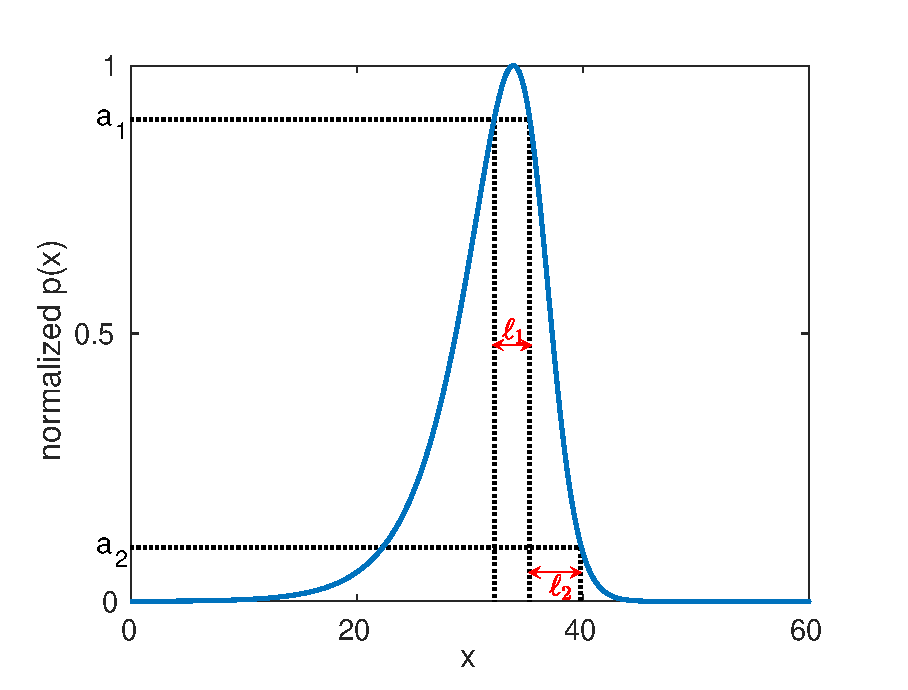
\includegraphics[scale=0.6]{plots/waveprofile.eps}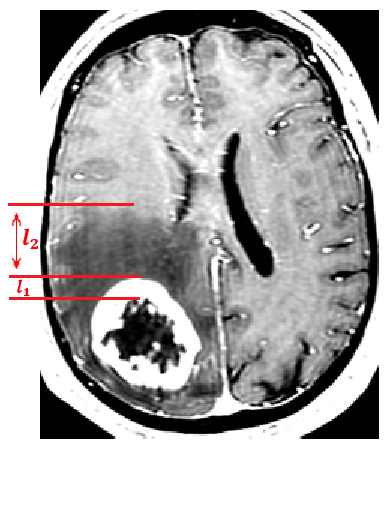
\includegraphics[scale=0.33]{plots/MR.png}
\end{center}
\caption{\label{fig:Match wid} Left: normalized wave profile generated by the model. Right: tumor profile seen in MR image. Parameter estimation is done by matching model-derived quantities, e.g., $\ell_1$ and $\ell_2$, to the corresponding image-derived ones. }

\end{figure}



\section{Results}
We first investigate the monotonicity of $f(\cdot)$ for some specific
choice of $g(w)$ and $\delta(w)$ because it is crucial for parameter
identifiability. Given our restrictions on $g(w)$ and $\delta(w)$,
the cumulative density function (cdf) of Beta distribution family
suits our purposes ($\delta(w)=1-cdf(w)$). By tweeting the scale
and shape of beta distribution we can get linear, sigmoid and concave
up/down curves (see left pane of Figure \ref{fig:beta =000026 f}).
It turns out that our framework is very robust to those choices, i.e.,
monotonicity of $f(\cdot$) is well preserved (right pane of Figure
\ref{fig:beta =000026 f}). As we can see, the sigmoid shaped $g(w)$
and $\delta(w)$ give larger range of $f(\cdot)$ and thus more flexibility
in parameter estimation. Moreover, sigmoid curves are believed to
be biological relevant (most enzymatic reaction rates have the same
shape with respect to reactant concentration). Therefore, we focus
on this choice and move on to find patient specific parameters using
their MR images. 

We parameterize our model with patient's data in which there is only
one MR scan before surgery. In Table \ref{tab:Patient-data-para}
we summarize the image-derived tumor radii and the corresponding parameters
estimated by the method introduced in the previous section. We observe
substantial variation of the parameters among individual patients. 

We compare our approximate quantities to those obtained from the numerical
solution of the model. As shown in Figure \ref{fig:comparison-to-numerical},
the approximated results match with numerical results well except
for some discrepancy for $L_{2}$ when $\hat{\rho}$ is small. It
is not a surprise since the approximation is based on assumption of
large $c=2\sqrt{\hat{\rho}}$ . Moreover, numerical approximation
of $L_{2}$ is prone to errors due to the fixed grid size and large
rate of change around the threshold of $L_{2}$. Overall, we are convinced
that our approximation is accurate for the parameter range arisen
from the image data. 

\begin{figure}
\begin{center}
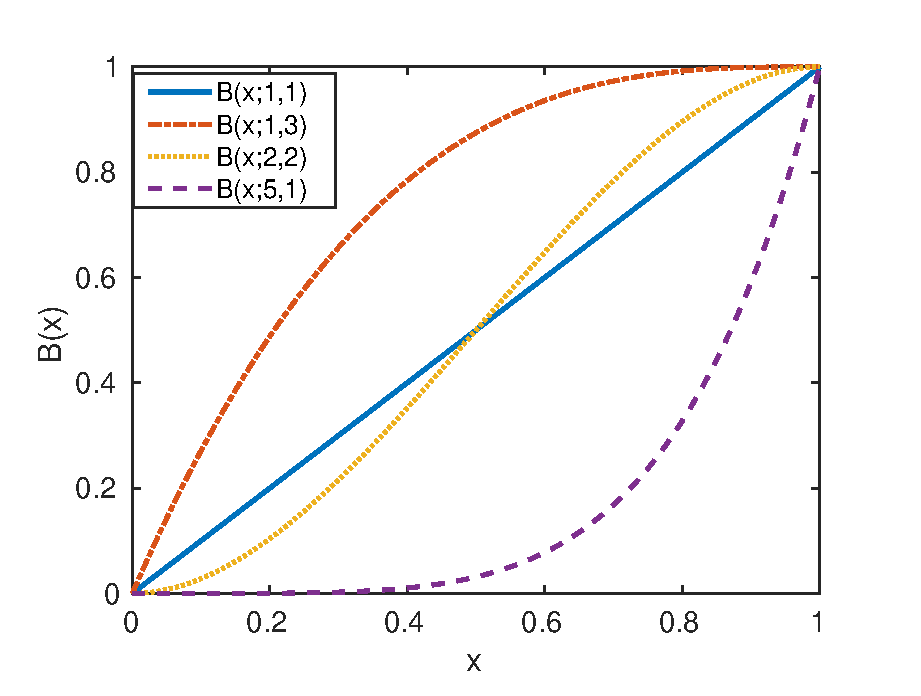
\includegraphics[scale=0.5]{plots/frhok/betas-new}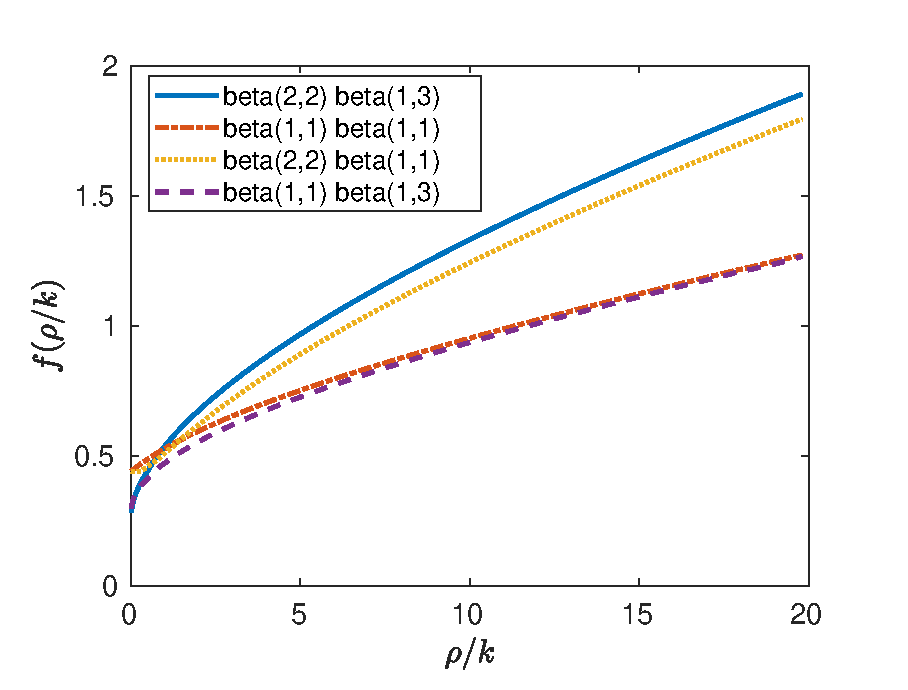
\includegraphics[scale=0.5]{plots/frhok/frhok-new}
\end{center}
\caption{\label{fig:beta =000026 f}Left: cdf of some beta distribution. These functions satisfy (\ref{eq:1st assumption})  and serve as reasonable candidates to phenomenologically represent biological response to limitation of growth factors. Right:
monotonicity of $f(\cdot)$ given different choices of $g(w)$ and $\delta(w)$ as indicated in the legend. All choices lead to monotonic function $f(\cdot)$ and hence identifiable parameters.}
\end{figure}

\begin{table}[H]
\begin{center}
\caption{\label{tab:Patient-data-para} Radii of equivalent tumor sphere derived
from T1 and T2 images and their corresponding estimated parameters.}
\begin{tabular}{ccccccc} \hline
Patient no. & $R_0$, mm & $R_1$, mm & $R_2$, mm & $D$, mm$^{2} $s$^{-1}$ & $\rho$, s$^{-1}$ & $k$, s$^{-1}$\\ \hline

1 & 14.87 & 15.24 & 15.83 & 0.2873 & 0.0529 & 0.0152 \\
2 & 20.73 & 22.87 & 20.35 & 0.9009 & 0.0462 & 0.0623 \\
3 & 27.77 & 26.96 & 19.83 & 0.108  & 0.0568 & 0.0107 \\
4 & 20.48 & 37.03 & 23.8  & 0.6747 & 0.0445 & 0.1342 \\
5 & 26.34 & 8.17  & 38.05 & 0.7374 & 0.0476 & 0.0426 \\
6 & 38.24 & 14.2  & 13.31 & 0.1057 & 0.0635 & 0.0041 \\
7 & 10.91 & 8.29  & 34.33 & 1.2655 & 0.046  & 0.0645 \\ \hline
\end{tabular}
\end{center}
%(Table body should be created by MS word table function; three-line table is preferred.)
\end{table}




\begin{figure}
\begin{center}
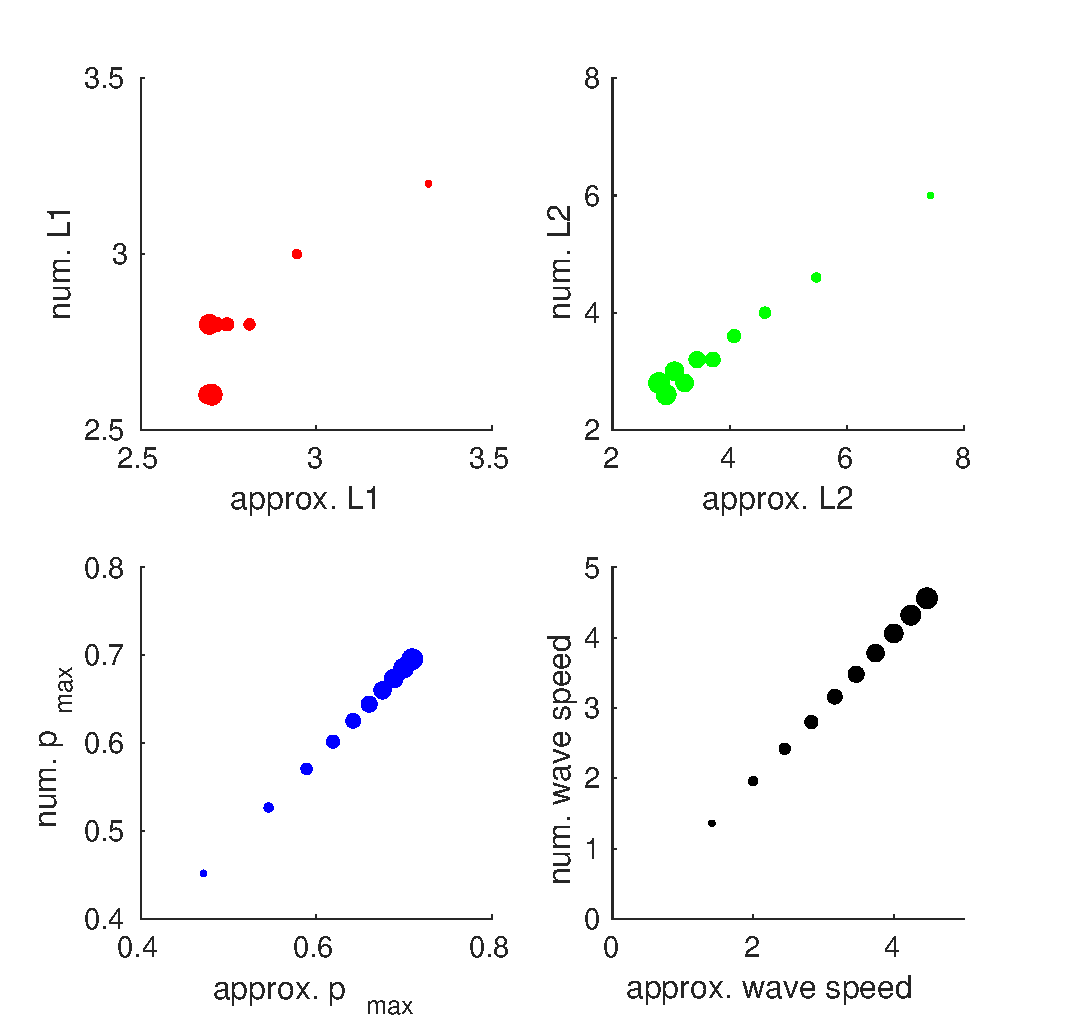
\includegraphics[scale=0.7]{plots/scatterplot-new}
\end{center}


\caption{\label{fig:comparison-to-numerical}Scatter plots of approximate wave
profile characteristics (on horizontal axis) verses the ones obtained
by numerical simulation (on vertical axis) for a range of $\hat{\rho}$
from 0.5 to 5 by incremental 0.5. The size the the dot corresponds
to the value of $\hat{\rho}$. The dots scatter closely to the diagonal line with slope 1, indicating agreement between the numerical solution and our approximation.}
\end{figure}
 

\section{Discussion}
The diffusion term in (\ref{eq:main}) falls into a general category
called cross diffusion \cite{Madzvamuse2017}, a phenomenon in which
the gradient in the concentration of one species can cause a flux
of another species. This type of cross diffusion considered here was
studied in a more general and theoretical context \cite{Sherratt2000}.
In \cite{Sherratt2001}, the authors justified the adoption of this
proportion-based cross diffusion in a tumor growth model by recognizing
that tumor cell migration is ``contact inhibited'', i.e., the presence
of one type of cell prevents the movements of the other. In other
words, the movements of one type of cell drags along other type of
cells with it. It is believed that this type of diffusion is more
realistic than simple linear diffusion (Fickian) in a sense that it
prevents unrealistic mixing of cells. Other types of density-dependent
diffusion are considered in modeling GBM migration \cite{Stepien2015a}.
Although a more complete picture of cell migration needs to include
mechanisms such as chemotaxis and haptotaxis, tumor growth is oftentimes
seen as diffusive and a careful choice of diffusion term is believed
to be sufficient to model cell migration in many cases. Although the
most accurate form of diffusion is debatable in the context of GBM,
we note that in our analysis the exact form of diffusion does not
matter since the second derivatives are dropped in (\ref{eq:1/c^2}).
The diffusion coefficient does play an important role in the linearized
wave head where it affects the wave speed, and in characteristic length
where its square root scales the space. Whereas the scale invariant
part of the wave profile is mostly determined by the exact form of
birth and death for which we did a thorough exploration. So we believe
that our model should capture the essence of the tumor morphology
revealed by MR images. 

Traveling wave solution is not uncommon in a reaction-diffusion system
and studies on this topic date back to \cite{FISHER1937}. Rigorous
proof of existence of traveling wave solution in a reaction-diffusion
system often leads to phase space analysis such as in \cite{Dunbar1983}.
Not only the high dimension but also the singularity represented in
the cross diffusion makes a proof a changeling task, which will the
the focus of future work. Nevertheless, the reduced system is reconcilable
to phase plane analysis and the orbit representing the traveling wave
solution can be identified (see appendix). 

Instead of having a lumped proliferation term as in \cite{Jackson2015a}
which only tracks net proliferation, our model treats birth and death
separately, making it possible to gauge the underlying total proliferation
of cancer cells. This is valuable information for personalized treatment
design since most chemotherapy and radiotherapy target proliferating
cells. Moreover, the structural information is also potential useful,
e.g., it may instruct drug dose so that the drug can perfuse through
the width of the proliferating rim. Research along this line has been
conducted using the PI model \cite{Kim2017}. We plan to investigate
along this line using our model in the future study. 

We recognize the possibility that the tumor is evolving over its course
of growth as the observed tumor profile at two different times is
not scale invariant. We suspect that the parameters of the model are
not constant over time. In this paper, we devise a method which uses
two MR images taken at two consecutive times before surgery, and our
method is feasible whether the two scans are consistent with invariant
tumor profile or not. It is straightforward to extend the current
method to make use of MR images taken at three or even more time points.
By updating parameters as more data is acquired, we are essentially
doing data assimilation. There has been research on applying full-fledged
data assimilation to cancer modeling \cite{Kostelich2011,McDaniel2013}.
Our method stands out being simple and computationally light-weighted.
In the case when only one per-surgery MR scan is available, we demonstrated
a way to estimate parameters involving mild and experimentally verifiable
assumptions. The major contributions of this paper is the novel way
to make use of scarce data which are the routinely available in clinical
settings. So we hope our method would offer wide and practical use
compared to large-scale computational models \cite{Eikenberry2009,Rutter2017},
which often focus on experimental data. 


%\section{Conclusion}

\section*{Acknowledgments}
The authors would like to thank Leslie Baxter and Leland Ho at Barrow
Neurological Institute for providing MR images. The work is supported
by an grant from Arizona Biomedical Research Center. \\

%\section*{Conflict of interest}

%\bibliographystyle{AIMS}
%\bibliography{ref}

\providecommand{\href}[2]{#2}
\providecommand{\arxiv}[1]{\href{http://arxiv.org/abs/#1}{arXiv:#1}}
\providecommand{\url}[1]{\texttt{#1}}
\providecommand{\urlprefix}{URL }
\begin{thebibliography}{10}

\bibitem{Canosa1973}
\newblock J.~Canosa,
\newblock {On a Nonlinear Diffusion Equation Describing Population Growth},
\newblock \emph{IBM Journal of Research and Development}, \textbf{17} (1973),
  307--313,
\newblock \urlprefix\url{http://ieeexplore.ieee.org/document/5391351/}.

\bibitem{Dunbar1983}
\newblock S.~Dunbar,
\newblock {Travelling wave solutions of diffusive Lotka-Volterra equations},
\newblock \emph{Journal of Mathematical Biology}, \textbf{17} (1983), 11--32,
\newblock \urlprefix\url{http://link.springer.com/10.1007/BF00276112}.

\bibitem{Eikenberry2009}
\newblock S.~E. Eikenberry, T.~Sankar, M.~C. Preul, E.~J. Kostelich, C.~J.
  Thalhauser and Y.~Kuang,
\newblock {Virtual glioblastoma: Growth, migration and treatment in a
  three-dimensional mathematical model},
\newblock \emph{Cell Proliferation}, \textbf{42} (2009), 511--528.

\bibitem{FISHER1937}
\newblock R.~A. Fisher,
\newblock {The wave of advance of advantageous genes},
\newblock \emph{Annals of Eugenics}, \textbf{7} (1937), 355--369,
\newblock
  \urlprefix\url{http://doi.wiley.com/10.1111/j.1469-1809.1937.tb02153.x}.

\bibitem{Gerlee2016}
\newblock P.~Gerlee and S.~Nelander,
\newblock {Travelling wave analysis of a mathematical model of glioblastoma
  growth},
\newblock \emph{Mathematical Biosciences}, \textbf{276} (2016), 75--81,
\newblock
  \urlprefix\url{https://www.sciencedirect.com/science/article/abs/pii/S0025556416000602?via{\%}3Dihub}.

\bibitem{Harley2014}
\newblock K.~Harley, P.~van Heijster, R.~Marangell, G.~J. Pettet and
  M.~Wechselberger,
\newblock {Existence of Traveling Wave Solutions for a Model of Tumor
  Invasion},
\newblock \emph{SIAM Journal on Applied Dynamical Systems}, \textbf{13} (2014),
  366--396,
\newblock \urlprefix\url{http://epubs.siam.org/doi/10.1137/130923129}.

\bibitem{Jackson2015a}
\newblock P.~R. Jackson, J.~Juliano, A.~Hawkins-Daarud, R.~C. Rockne and K.~R.
  Swanson,
\newblock {Patient-Specific Mathematical Neuro-Oncology: Using a Simple
  Proliferation and Invasion Tumor Model to Inform Clinical Practice},
\newblock \emph{Bulletin of Mathematical Biology}, \textbf{77} (2015),
  846--856,
\newblock \urlprefix\url{http://link.springer.com/10.1007/s11538-015-0067-7}.

\bibitem{Kim2017}
\newblock M.~Kim, J.~Kotas, J.~Rockhill, M.~Phillips, M.~Kim, J.~Kotas,
  J.~Rockhill and M.~Phillips,
\newblock {A Feasibility Study of Personalized Prescription Schemes for
  Glioblastoma Patients Using a Proliferation and Invasion Glioma Model},
\newblock \emph{Cancers}, \textbf{9} (2017), 51,
\newblock \urlprefix\url{http://www.mdpi.com/2072-6694/9/5/51}.

\bibitem{Kostelich2011}
\newblock E.~J. Kostelich, Y.~Kuang, J.~M. McDaniel, N.~Z. Moore, N.~L.
  Martirosyan and M.~C. Preul,
\newblock {Accurate state estimation from uncertain data and models: an
  application of data assimilation to mathematical models of human brain
  tumors},
\newblock \emph{Biology Direct}, \textbf{6} (2011), 64,
\newblock
  \urlprefix\url{http://biologydirect.biomedcentral.com/articles/10.1186/1745-6150-6-64}.

\bibitem{Kuang}
\newblock Y.~Kuang, J.~D. Nagy and S.~E. Eikenberry,
\newblock \emph{{Introduction to mathematical oncology}},
\newblock Chapman and Hall/CRC.

\bibitem{Madzvamuse2017}
\newblock A.~Madzvamuse, R.~Barreira and A.~Gerisch,
\newblock {Cross-Diffusion in Reaction-Diffusion Models: Analysis, Numerics,
  and Applications},
\newblock Springer, Cham, 2017,
\newblock 385--392,
\newblock
  \urlprefix\url{http://link.springer.com/10.1007/978-3-319-63082-3{\_}61}.

\bibitem{GBMreview}
\newblock N.~L. Martirosyan, E.~M. Rutter, W.~L. Ramey, E.~J. Kostelich,
  Y.~Kuang and M.~C. Preul,
\newblock {Mathematically modeling the biological properties of gliomas: A
  review},
\newblock \emph{Mathematical Biosciences and Engineering}, \textbf{12} (2015),
  879--905,
\newblock \urlprefix\url{http://www.ncbi.nlm.nih.gov/pubmed/25974347
  http://www.aimsciences.org/journals/displayArticlesnew.jsp?paperID=11020}.

\bibitem{McDaniel2013}
\newblock J.~McDaniel, E.~Kostelich, Y.~Kuang, J.~Nagy, M.~C. Preul, N.~Z.
  Moore and N.~L. Matirosyan,
\newblock {Data Assimilation in Brain Tumor Models},
\newblock Springer, New York, NY, 2013,
\newblock 233--262,
\newblock
  \urlprefix\url{http://link.springer.com/10.1007/978-1-4614-4178-6{\_}9}.

\bibitem{Neal2013}
\newblock M.~L. Neal, A.~D. Trister, T.~Cloke, R.~Sodt, S.~Ahn, A.~L. Baldock,
  C.~A. Bridge, A.~Lai, T.~F. Cloughesy, M.~M. Mrugala, J.~K. Rockhill, R.~C.
  Rockne and K.~R. Swanson,
\newblock {Discriminating Survival Outcomes in Patients with Glioblastoma Using
  a Simulation-Based, Patient-Specific Response Metric},
\newblock \emph{PLoS ONE}, \textbf{8} (2013), e51951,
\newblock \urlprefix\url{https://dx.plos.org/10.1371/journal.pone.0051951}.

\bibitem{Norden2006}
\newblock A.~D. Norden and P.~Y. Wen,
\newblock {Glioma therapy in adults},
\newblock \emph{The neurologist}, \textbf{12} (2006), 279--92,
\newblock \urlprefix\url{http://www.ncbi.nlm.nih.gov/pubmed/17122724}.

\bibitem{Rutter2017}
\newblock E.~M. Rutter, T.~L. Stepien, B.~J. Anderies, J.~D. Plasencia, E.~C.
  Woolf, A.~C. Scheck, G.~H. Turner, Q.~Liu, D.~Frakes, V.~Kodibagkar,
  Y.~Kuang, M.~C. Preul and E.~J. Kostelich,
\newblock {Mathematical Analysis of Glioma Growth in a Murine Model},
\newblock \emph{Scientific reports}, \textbf{7} (2017), 2508,
\newblock
  \urlprefix\url{http://www.ncbi.nlm.nih.gov/pubmed/28566701{\%}5Cnhttp://www.pubmedcentral.nih.gov/articlerender.fcgi?artid=PMC5451439}.

\bibitem{Sherratt2000}
\newblock J.~A. Sherratt,
\newblock {Wavefront propagation in a competition equation with a new motility
  term modelling contact inhibition between cell populations},
\newblock \emph{Proceedings of the Royal Society of London. Series A:
  Mathematical, Physical and Engineering Sciences}, \textbf{456} (2000),
  2365--2386,
\newblock
  \urlprefix\url{http://www.royalsocietypublishing.org/doi/10.1098/rspa.2000.0616}.

\bibitem{Sherratt2001}
\newblock J.~A. Sherratt and M.~A. Chaplain,
\newblock {A new mathematical model for avascular tumour growth},
\newblock \emph{Journal of Mathematical Biology}, \textbf{43} (2001), 291--312,
\newblock \urlprefix\url{http://link.springer.com/10.1007/s002850100088}.

\bibitem{Stepien2015a}
\newblock T.~L. Stepien, E.~M. Rutter and Y.~Kuang,
\newblock {A data-motivated density-dependent diffusion model of in vitro
  glioblastoma growth.},
\newblock \emph{Mathematical biosciences and engineering : MBE}, \textbf{12}
  (2015), 1157--72,
\newblock \urlprefix\url{http://www.ncbi.nlm.nih.gov/pubmed/26775861}.

\bibitem{Stepien2018}
\newblock T.~L. Stepien, E.~M. Rutter and Y.~Kuang,
\newblock {Traveling Waves of a Go-or-Grow Model of Glioma Growth},
\newblock \emph{SIAM Journal on Applied Mathematics}, \textbf{78} (2018),
  1778--1801,
\newblock \urlprefix\url{https://epubs.siam.org/doi/10.1137/17M1146257}.

\bibitem{Swanson2011}
\newblock K.~R. Swanson, R.~C. Rockne, J.~Claridge, M.~A. Chaplain, E.~C.
  Alvord and A.~R.~A. Anderson,
\newblock {Quantifying the Role of Angiogenesis in Malignant Progression of
  Gliomas: In Silico Modeling Integrates Imaging and Histology},
\newblock \emph{Cancer Research}, \textbf{71} (2011), 7366--7375,
\newblock \urlprefix\url{http://www.ncbi.nlm.nih.gov/pubmed/21900399
  http://www.pubmedcentral.nih.gov/articlerender.fcgi?artid=PMC3398690
  http://cancerres.aacrjournals.org/cgi/doi/10.1158/0008-5472.CAN-11-1399}.

\bibitem{Swanson2008}
\newblock K.~R. Swanson, R.~C. Rostomily and E.~C. Alvord,
\newblock {A mathematical modelling tool for predicting survival of individual
  patients following resection of glioblastoma: a proof of principle},
\newblock \emph{British Journal of Cancer}, \textbf{98} (2008), 113--119,
\newblock \urlprefix\url{http://www.nature.com/articles/6604125}.

\end{thebibliography}


%For more questions regarding reference style, please refer to the \href{http://www.ncbi.nlm.nih.gov/books/NBK7256/}{Citing Medicine}.

\section*{Supplementary}

We perform phase plane ($w$-$p$ plane, see Figure \ref{fig:pp}) analysis of (\ref{eq:pp system})
to show the existence of a trajectory that starts from $(1,0)$ and
ends at $(w^{*},0)$ where $w^{*}\ge0$ if (\ref{eq:1st assumption})
are satisfied. The Jacobian matrix at (0,1) is 
\begin{equation}
\begin{bmatrix}
\hat{\rho} & 0\\
-\hat{\rho} & 0
\end{bmatrix}.
\end{equation}
It follows that $(1,0)$ is an unstable fixed point
and the trajectory starting here has slope $-1$ which is the direction
of the unstable manifold. Moreover 
\[
\frac{d^{2}p}{dw^{2}}=\frac{\delta'(w)g(w)-\delta(w)g'(w)}{\hat{\rho} g(w)^{2}}<0
\]
for $w\in(0,1)$ because of the assumptions (\ref{eq:1st assumption}) we proposed on $g(w)$ and $\delta(w)$.
It follows that the trajacory must remain below the line $p=1-w$.
Assuming $g(w)$ and $\delta(w)$ are continuous, there must be a
$w^{\dagger}\in(0,1)$ such that $\rho g(w^{\dagger})=\delta(w^{\dagger})$.
For $w>w^{\dagger}$, the trajectory has positive slope and hence
heading down to the $w$-axis. Since $\frac{dw}{dz}\vert_{w=0}=0$,
the trajectory cannot cross $p$-axis. Thus it must intersect the
$w$-axis at some pont $w^{*}\in(0,w^{\dagger}).$ 

\end{document}
